\chapter{Command Pattern}

\section{Định nghĩa}
\begin{itemize}
\item Command Pattern là một trong những Pattern thuộc nhóm hành vi (Behavior Pattern). Nó cho phép chuyển yêu cầu thành đối tượng độc lập, có thể được sử dụng để tham số hóa các đối tượng với các yêu cầu khác nhau như log, queue (undo/redo), transtraction. Nói cách khác, Command Pattern cho phép tất cả những request gửi đến object được lưu trữ trong chính object đó dưới dạng một object Command. Khái niệm Command Object giống như một class trung gian được tạo ra để lưu trữ các câu lệnh và trạng thái của object tại một thời điểm nào đó.
\item Command dịch ra nghĩa là ra lệnh. Commander nghĩa là chỉ huy, người này không làm mà chỉ ra lệnh cho người khác làm. Như vậy, phải có người nhận lệnh và thi hành lệnh. Người ra lệnh cần cung cấp một class đóng gói những mệnh lệnh. Người nhận mệnh lệnh cần phân biệt những interface nào để thực hiện đúng mệnh lệnh.
\item Command Pattern còn được biết đến như là Action hoặc Transaction.
\end{itemize}

\section{Mục đích sử dụng}
\begin{itemize}
\item Tham số hóa các đối tượng theo một hành động thực hiện
\item Tạo và thực thi các yêu cầu vào các thời điểm khác nhau
\item Hỗ trợ tính năng undo, log, callback hoặc transaction
\end{itemize}

\section{Mô hình cấu trúc}
\begin{center}
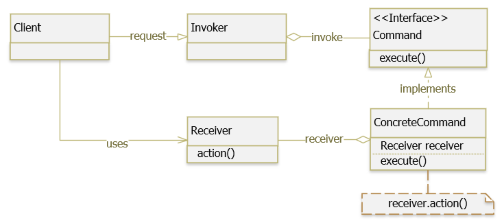
\includegraphics{GALLEYS/images/chapter7/diagram}
\end{center}
Các thành phần:
\begin{itemize}
\item Command : là một interface hoặc abstract class, chứa một phương thức trừu tượng thực thi (execute) một hành động (operation). Request sẽ được đóng gói dưới dạng Command.
\item ConcreteCommand : là các implementation của Command. Định nghĩa một sự gắn kết giữa một đối tượng Receiver và một hành động. Thực thi execute() bằng việc gọi operation đang hoãn trên Receiver. Mỗi một ConcreteCommand sẽ phục vụ cho một case request riêng.
\item Client : tiếp nhận request từ phía người dùng, đóng gói request thành ConcreteCommand thích hợp và thiết lập receiver của nó.
\item Invoker : tiếp nhận ConcreteCommand từ Client và gọi execute() của ConcreteCommand để thực thi request.
\item Receiver : đây là thành phần thực sự xử lý business logic cho case request. Trong phương execute() của ConcreteCommand chúng ta sẽ gọi method thích hợp trong Receiver.
\end{itemize}
Như vậy, Client và Invoker sẽ thực hiện việc tiếp nhận request. Còn việc thực thi request sẽ do Command, ConcreteCommand và Receiver đảm nhận.\\

Để có thể hiểu rõ hơn, chúng ta sẽ xét ví dụ mà Command Pattern được trong ứng dụng mở tài khoản ngân hàng: Một hệ thống ngân hàng cung cấp ứng dụng cho khách hàng (client) có thể mở (open) hoặc đóng (close) tài khoản trực tuyến. Hệ thống này được thiết kế theo dạng module, mỗi module sẽ thực hiện một nhiệm vụ riêng của nó, chẳng hạn mở tài khoản (OpenAccount), đóng tài khoản (CloseAccount). Do hệ thống không biết mỗi module sẽ làm gì, nên khi có yêu cầu client (chẳng hạn clickOpenAccount, clickCloseAccount), nó sẽ đóng gói yêu cầu này và gọi module xử lý. Chúng ta có thể hình dung thông qua hình dưới đây:
\begin{center}
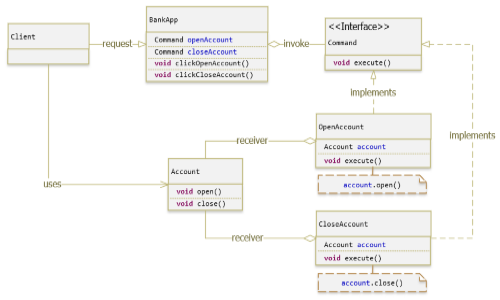
\includegraphics{GALLEYS/images/chapter7/example}
\end{center}
Ứng dụng của chúng ta bao gồm các lớp xử lý sau:
\begin{itemize}
\item Account : là một request class.
\item Command : là một interface của Command Pattern, cung cấp phương thức execute().
\item OpenAccount, CloseAccount : là các ConcreteCommand, cài đặt các phương thức của Command, sẽ thực hiện các xử lý thực tế.
\item BankApp : là một class, hoạt động như Invoker, gọi execute() của ConcreteCommand để thực thi request.
\item Client : tiếp nhận request từ phía người dùng, đóng gói request thành ConcreteCommand thích hợp và gọi thực thi các Command.
\end{itemize}
Cụ thể các lớp của chúng ta sẽ được thiết kế như sau:\\
\textbf{Account.java}:
\begin{center}
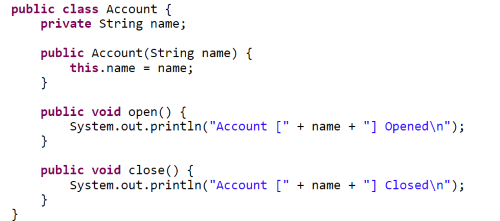
\includegraphics{GALLEYS/images/chapter7/code1}
\end{center}
\textbf{Command.java}
\begin{center}
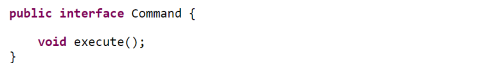
\includegraphics{GALLEYS/images/chapter7/code2}
\end{center}
\textbf{OpenAccount.java}
\begin{center}
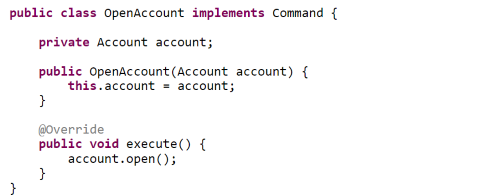
\includegraphics{GALLEYS/images/chapter7/code3}
\end{center}
\textbf{CloseAccount.java}
\begin{center}
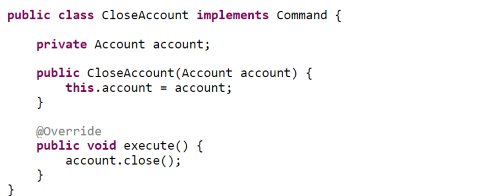
\includegraphics{GALLEYS/images/chapter7/code4}
\end{center}
\textbf{BankApp.java}
\begin{center}
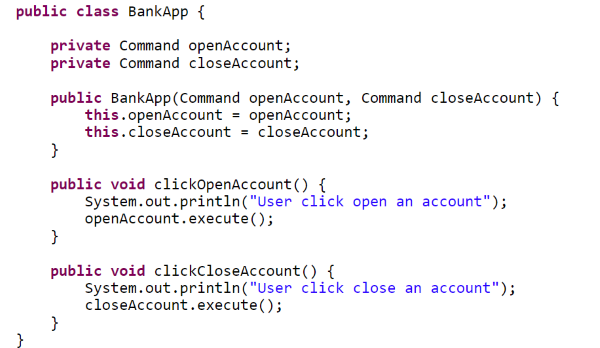
\includegraphics{GALLEYS/images/chapter7/code5}
\end{center}
\textbf{Client.java}
\begin{center}
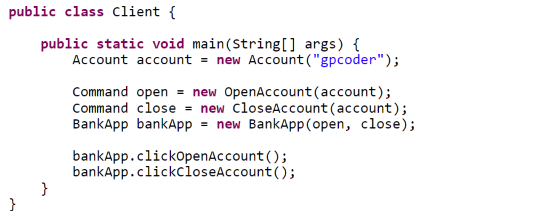
\includegraphics{GALLEYS/images/chapter7/code6}
\end{center}
\textbf{Và cuối cùng là output của chương trình}
\begin{center}
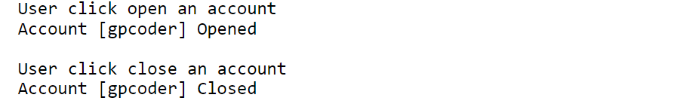
\includegraphics{GALLEYS/images/chapter7/code7}
\end{center}

\section{Command Pattern trong thực tế}
Command Pattern được ứng dụng khá nhiều trong thực tế, có thể kể đến vài trường hợp áp dụng Command Pattern:
\begin{itemize}
	\item Graphical User Interface (GUI) - Giao diện đồ họa người dùng: Trong GUI và các mục menu, chúng ta sử dụng Command Pattern. Bằng cách nhấp vào một nút nào đó, chúng ta có thể đọc thông tin hiện tại của GUI và thực hiện một hành động tương ứng.
	\item Marco Recording (Ghi Macro): Nếu mỗi hành động của người dùng được triển khai dưới dạng một mệnh lệnh (Command) riêng biệt, chúng ta có thể ghi lại tất cả các hành động của người dùng trong Macro dưới dạng một chuỗi các mệnh lệnh. Chúng ta có thể sử dụng chuỗi này để triển khai tính năng "alPhát lại" (Playback). Bằng cách này, Macro có thể tiếp tục thực hiện cùng một nhóCommandm hành động với mỗi lần phát lại.
	\item Multi-step Undo (Hoàn tác nhiều bước): Khi mỗi bước được ghi lại dưới dạng một mệnh lệnh (Command), chúng ta có thể sử dụng nó để triển khai tính năng Undo (Hoàn tác) mà mỗi bước có thể hoàn tác. Nó được sử dụng trong các trình soạn thảo văn bản như MS-Word.
	\item Networking (Kết nối mạng): Chúng ta cũng có thể gửi một mệnh lệnh (Command) hoàn chỉnh qua mạng tới một máy từ xa nơi tất cả các hành động được gói gọn trong một mệnh lệnh (Command) được thực thi.
	\item Progress Bar (Thanh tiến trình): Chúng ta có thể triển khai một quy trình cài đặt dưới dạng một chuỗi các mệnh lệnh (Command). Mỗi mệnh lệnh cung cấp thời gian ước tính. Khi chúng ta thực hiện quy trình cài đặt, với mỗi mệnh lệnh chúng ta có thể hiển thị thanh tiến trình.
	\item Wizard: Trong quy trình wizard, chúng ta có thể triển khai các bước dưới dạng các mệnh lệnh. Mỗi bước có thể có nhiệm vụ phức tạp mà chỉ được thực hiện trong một lệnh.
	\item Transactions: Trong một mã hành vi transactional có nhiều tác vụ/cập nhật. Khi tất cả các nhiệm vụ được thực hiện thì chỉ có transaction được cam kết. Nếu không, chúng tôi phải khôi phục transaction (rollback the transaction). Trong một kịch bản như vậy, mỗi bước được thực hiện dưới dạng mệnh lệnh (Command) riêng biệt.
\end{itemize}
